\chapter{Dependence on the number of modes}

Due to the energy mode cutoff in the decomposition of the field when calculating the charge density in Equation \eqref{eq:Hadamard-vacuum-polarization}, it is important to study the dependence of the self-consistent fields on the number of modes considered. In calculating the solutions to the Klein-Gordon-Maxwell equations \eqref{eq:KG-equation}, the main quantity of interest depending on the mode expansion is the backreacting electrostatic potential $A_0^\text{br}(x)$. 

Figure \ref{fig:A0-mode-dependence} shows the dependence of the induced backreacting electrostatic potential $A_0^\text{br}(z)$ parameterized by the number of modes considered in the expansion of the field. 
For low $\lambda$ values, the system is expected to behave perturbatively. We therefore show for reference the perturbative backreacting potential, i.e. the second integral the perturbative vacuum approximation shown in Equation \eqref{eq:perturbative-vacuum-polarization}. We only observe a single curve since different potentials almos perfectly overlap. 

%It should be noted, that the vacuum polarization $\rho$ from which $A_0^\text{br}$ is calculated, is not 

As a finer measure of the changes in the potential $A_0^\text{br}$, the right panel of \ref{fig:A0-mode-dependence} provides the potential $A_0^\text{br}(z)$ evaluated at $z=1$, again as a function of the modes considered in the expansion. We here see a small variation of the order of 1\%, and a converging behavior for higher number of modes, as should be expected. Again, the value of the perturbative potential is shown for reference.
\begin{figure}
\begin{subfigure}{0.5\textwidth}
    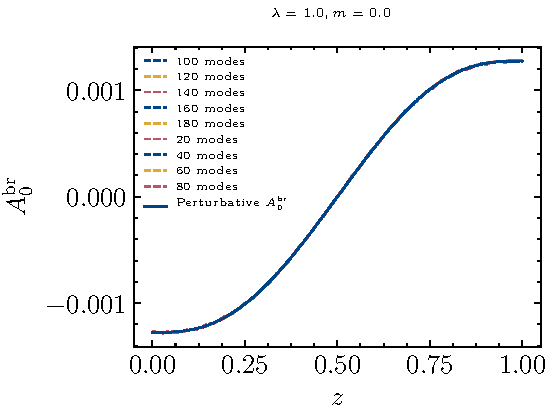
\includegraphics[width=\linewidth]{figures/dirichlet/A0InducedComparison.pdf}
\end{subfigure}
\begin{subfigure}{0.5\textwidth}
    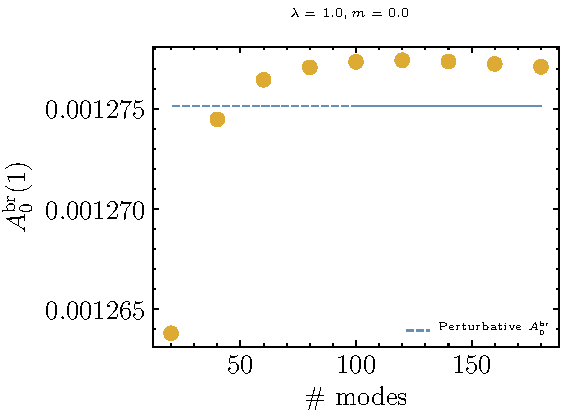
\includegraphics[width=\linewidth]{figures/dirichlet/A0(1) mode comparison.pdf}
\end{subfigure}
\caption{In the left panel, the backreacting electrostatic potential $A_0^\text{br}(z)$ parameterized by the number of modes considered in the expansion for the massless Klein-Gordon field with Dirichlet boundary conditions and a background electric field of strength $\lambda=1$.
%The vacuum polarization with respect to which the potential is calculated is not smoothed.
Additionally, the induced electrostatic potential corresponding to the vacuum polarization calculated in the perturbative approximation, following equation \eqref{eq:perturbative-vacuum-polarization}. In the right panel, a "zoom-in" at the right boundary $z=1$ displaying the small variations of the potential for different number of modes, and as reference, the value for the perturbative electrostatic potential.}
\label{fig:A0-mode-dependence}
\end{figure}